\documentclass[12pt, a4paper]{article}
\usepackage[utf8]{inputenc}

% Font
\usepackage{MinionPro}
\input glyphtounicode
\pdfgentounicode=1
\usepackage{microtype}
\usepackage[super]{nth}
\usepackage{csquotes}

% Format
\setlength{\parindent}{0.5in}
\setcounter{secnumdepth}{0}

% Language
\usepackage[american]{babel}

% Links
\usepackage[colorlinks=true, linkcolor=black, urlcolor=black, citecolor=black]{hyperref} 

% Figures
\usepackage{graphicx}
\usepackage[small, labelfont=it, labelsep=period]{caption}

% Tables
\usepackage{booktabs}
\usepackage{tabularx}

% References
\usepackage[style=apa]{biblatex}
\DeclareSourcemap{
  \maps[datatype=bibtex]{
    \map{
      \pertype{book}
      \step[fieldset=location, null]
      \step[fieldset=address, null]
    }
    \map{
      \pertype{incollection}
      \step[fieldset=location, null]
      \step[fieldset=address, null]
    }
  }
}
\addbibresource{references.bib}
\renewcommand*{\bibfont}{\small}

% Frontmatter
\title{Intergroup contact fosters\\more inclusive social identities\thanks{Reimer, N. K., Kamble, S. V., Schmid, K., \& Hewstone, M. (in press). Intergroup contact fosters more inclusive social identities. \textit{Group Processes \& Intergroup Relations}. \href{https://doi.org/10.31234/osf.io/zcgwt}{https://doi.org/10.31234/osf.io/zcgwt}}}
\date{April 6, 2020}

\begin{document}

\maketitle

\begin{abstract}
\noindent We examined how people construct their social identities from multiple group memberships---and whether intergroup contact can reduce prejudice by fostering more inclusive social identities. South Indian participants ($N = 351$) from diverse caste backgrounds viewed 24 identity cards, each representing a person with whom participants shared none, one, two, or all of three group memberships (caste, religion, nationality). Participants judged each person as “us” or “not us”, showing whom they included in their ingroup, and whom they excluded. Participants tended to exclude caste and religious minorities, replicating persistent social divides. Bridging these divides, cross-group friendship was associated with more inclusive identities which, in turn, were associated with more positive relations between an advantaged, an intermediate, and a disadvantaged caste group. Negative contact was associated with less inclusive identities. Contact and identity processes, however, did not affect entrenched opposition to (or undermine support for) affirmative action in advantaged and disadvantaged groups.\\[1ex]
\noindent {\footnotesize \textbf{Keywords:} intergroup contact, social identity, multiple categorization, intergroup relations, interminority relations, perceived discrimination, affirmative action}
\end{abstract}

\noindent How we feel about and act toward others depends on whom we consider “us” and “them”---that is, whom we include in, and exclude from, our ingroup (for a review, see \nptextcite{reimer_self-categorization_2020}).  In some situations, this distinction rests on one salient categorization, for example, someone's nationality at an international border. In diverse societies, however, this distinction often depends on multiple, overlapping group memberships. Individuals differ in how they construct their ingroup from these group memberships. Some espouse narrow definitions of who is “us” and “them”, while others adopt more inclusive identities. Many Americans, for example, associate being American with being White American \parencite{devos_american_2005}. This suggests that whom Americans consider “us” and “them” might depend on someone's race \emph{and} nationality. In this paper, we examine how people construct their social identities from multiple group memberships---and whether intergroup contact can reduce prejudice by fostering more inclusive social identities. We use a novel method to study social identification across multiple social categories and to examine possible antecedents (intergroup contact, social dominance orientation) and consequences (intergroup attitudes, intergroup threat, support for affirmative action) of more inclusive identities.

\begin{figure*}
\centering
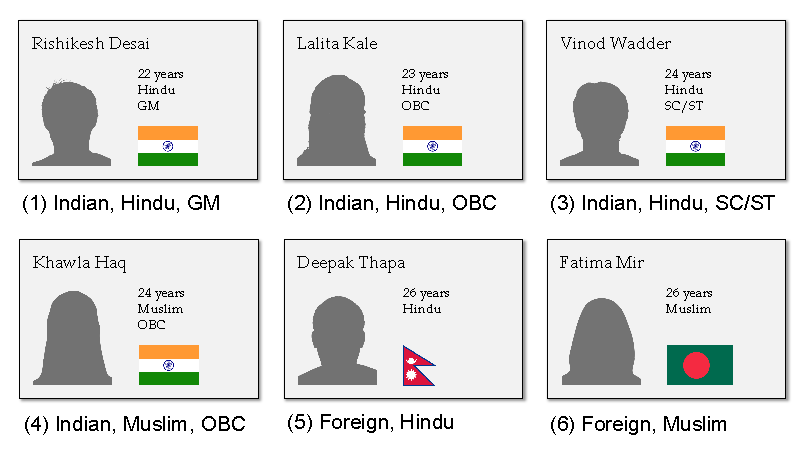
\includegraphics[scale=1]{../figures/figure-1}
\caption{
Schematic representations of social identity structures \protect\parencite{roccas_social_2002}, ordered by their social identity inclusiveness \protect\parencite{van_dommelen_construing_2015}. Shaded regions represent the groups which a participant has to categorize as “us” to be assigned that structure. An Indian Hindu, for example, might consider only people who share their nationality, religion, and caste as ingroup members (\emph{intersection}). Someone else might consider all their fellow Indians, whatever their religion or caste, as ingroup members (\emph{dominance}). Another person might consider anyone who shares their nationality or religion as ingroup members (\emph{merger}).
}
\label{fig:f1}
\end{figure*}

Social psychologists highlighted the importance of considering two \parencite{berry_immigration_1997, crisp_multiple_2007, dovidio_commonality_2009} or more \parencite{roccas_social_2002} social categories for understanding intergroup relations. \textcite{crisp_multiple_2007} reviewed evidence that we tend to have more favourable attitudes towards people with whom we share some, but not all, group memberships than towards people with whom we do not share any group memberships. \textcite{gaertner_reducing_2000} showed that espousing a more inclusive common ingroup identity (e.g., Indian) over a narrower identity (e.g., Hindu, Muslim) can extend the benefits of ingroup favouritism to outgroup members and thus reduce intergroup bias. \textcite{roccas_social_2002} recognized that, though we all hold multiple overlapping group memberships, we differ in how we construct our social identities from these group memberships. Broadly, these perspectives recognize that we are part of multiple overlapping groups; that we use these group memberships to construct a subjective sense of who is “us” and “them”; and that espousing more inclusive social identities can reduce prejudice and discrimination.

Diverse societies confront their members with the decision of which intersections of various group memberships to include in their subjective ingroup. One Indian Hindu, for example, might constrict their ingroup to people of the same nationality, religion, and caste. Another Indian Hindu might consider all Indians, whatever their religion or caste, as ingroup members (see Figure~\ref{fig:f1}). Past research \parencite{van_dommelen_construing_2015} indeed observed substantial individual differences in whom participants considered “us” and “not us”. Some participants espoused more inclusive social identities---that is, they included more people in their subjective ingroup. Other participants espoused less inclusive social identities---that is, they included fewer people in their subjective ingroup. All participants, however, belonged to the same disadvantaged minority group. Past research thus provided evidence for individual differences, but did not examine group differences in whom people consider “us” and “not us”.

\printbibliography

\end{document}
